\documentclass[letterpaper,oneside,12pt]{article}%twocolumn;titlepage(separate title page)
\usepackage{pslatex}                %Times New Roman Font; Improves on-screen readability; preferred to using times package
\usepackage[margin=1in]{geometry}   %1in 'uniform' margin (with oneside)
\usepackage{color}
\usepackage{amsmath}
\usepackage{amsfonts}
\usepackage{enumitem}
\usepackage{optprog}
\usepackage{url}
\usepackage{bm}
\usepackage{lscape}
\usepackage{tikz}
\setcounter{MaxMatrixCols}{20}
%\setlength{\headsep}{0in}           %Distance from bottom of header to the body of text on a page.
\newcommand{\rem}[1]{}

\DeclareMathOperator{\conv}{conv}
\DeclareMathOperator*{\proj}{proj}

\newcommand{\Sum}{\displaystyle \sum}
\newcommand{\blu}{\color{blue}}
\newcommand{\bla}{\color{black}}
\begin{document}
\noindent\fbox{%
	\parbox{\textwidth}{%
		\begin{center}
		\textbf{\large{SA405 -- Exam 2 Practice}}
		\end{center}
	}%
}

\bigskip

{
\blu
Solution
}

\begin{enumerate}
\item US NorthWest plans to install fiber in a metro area network that is expected to experience increased demand due to the opening of a large manufacturing facility.  The Central Offices (COs) in the network are represented by vertices in the graph below.  The edges in the graph represent the possible fiber paths linking the COs.  The number on edge $(i,j)$ represents the cost $c_{ij}$ (in \$1000) of installing fiber between COs $i$ and $j$.

\begin{center}
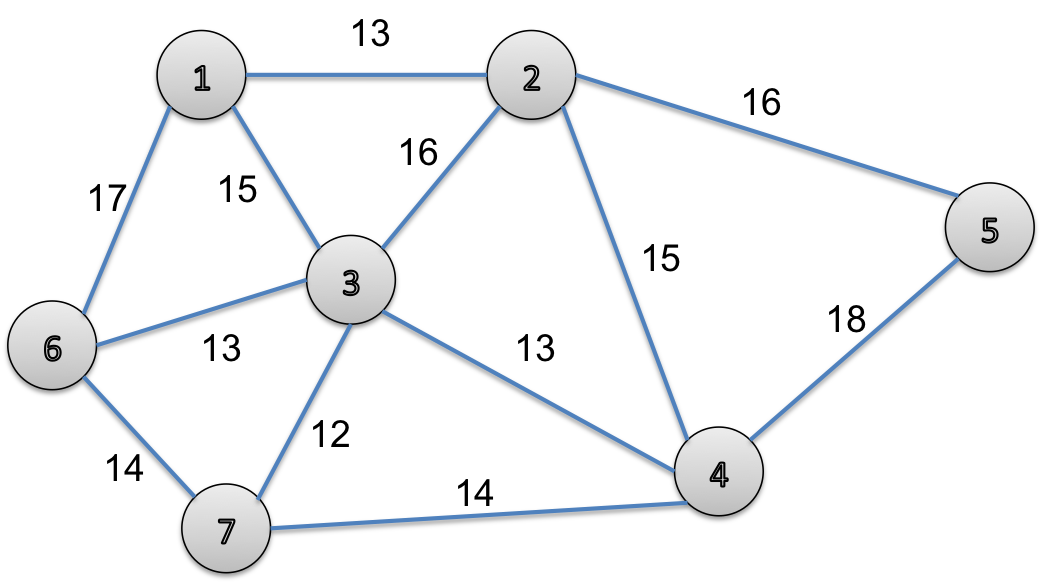
\includegraphics[width = .5\textwidth]{uswest_network}
\end{center}

\begin{enumerate}
\item Write an integer program in abstract form that provides the collection of edges that will minimize the cost of connecting all the central offices in the network via a fiber spanning tree.  Be sure to define any notation used, and to describe the purpose of each type of constraint.

{ \blu
\textbf{\underline{Sets}} \\
Let $E$ be the set of edges \\
Let $V$ be the set of vertices

\textbf{\underline{Decision Variables}} \\

Let $x_{i,j} = 1$ if edge $(i,j)$ is included in a spanning tree for all $(i,j) \in E$.

\textbf{\underline{Parameters}} \\

Let $c_{i,j}$ be the cost of edge $(i,j)$ for all $(i,j) \in E$

\begin{optprog*}
\text{min} & \objective{ \sum_{(i,j) \in E} c_{i,j} x_{i,j}  }\\
st & \sum_{(i,j) \in E: i = n, j = n} x_{i,j} & \geq  & 1 &  \text{for $n \in V$} \\
   & \sum_{(i,j) \in E} x_{i,j} & = & |V| - 1 \\
   & \sum_{(i,j) \in E: i \in S, j \in S} x_{i,j} & \leq & |S| - 1 & \text{for all $S \in V$} \\
   & x_{i,j} & \in & \{0,1\} 
\end{optprog*}

}

\item  In concrete form, write all of the constraints required to ensure that no cycle of any length is present among the nodes 1, 2, 3, and 4. 
{
\blu

Let $S_1 = \{1,2,3\}$ \\
Let $S_2 = \{1,2,4\}$ \\
Let $S_3 = \{1,3,4\}$ \\
Let $S_4 = \{2,3,4\}$ \\
Let $S_5 = \{1,2,3,4\}$ \\

We get:

\begin{optprog*}
& x_{1,2} + x_{1,3} + x_{2,3} & \leq & 2 \\
& x_{1,2} + x_{1,4} + x_{2,4} & \leq & 2 \\
& x_{1,3} + x_{1,4} + x_{3,4} & \leq & 2 \\
& x_{2,3} + x_{2,4} + x_{3,4} & \leq & 2 \\
& x_{1,2} + x_{1,3} + x_{1,4} + x_{2,3} + x_{2,4} + x_{3,4} & \leq & 3 \\
\end{optprog*}
}


\item  If this were a slightly larger problem, one of the sets of constraints in your abstract model from part (a) would need to be added iteratively.  
\begin{enumerate}
\item  Which set of constraints is this?

{ \blu

The subtour elimination constraints
}

\item  Explain why it does not work to add all of those constraints at once.
{
\blu

There are an exponential number of these constraints, if we add them all at the beginning the size of the problem will explode and it will not be solvable.
}
\item  Sketch a non-spanning-tree solution that is possible if these constraints are not included, and write out the constraint of this type that you would need to add to prevent this subgraph from occuring in the next iteration.

{
\blu

There's many examples. Suppose you get the solution 1-2-3-4 and 5-6-7 which results in 2 cycles. This solution satisfies the other constraints of the problem. You can eliminate this by writing:

Let $S_1 = \{1,2,3,4\}$\\
Let $S_2 = \{5,6,7\}$\\

Then including the constraint
\[
\sum_{(i,j) \in E: i \in S, j \in S} x_{i,j} \leq |S| - 1
\] for each of the two sets.

}

\end{enumerate}
\item The modeling team learns that city ordinances require that if link $(3,7)$ is built, then neither $(1,2)$ nor $(3,4)$ may be built.  Write a constraint to model this new requirement.

{
\blu

We want a constraint that says if $x_{3,7} = 1$ then $x_{1,2}$ and $x_{3,4} $ must both be $=0$. '

\[
2x_{3,7}  \leq (1-x_{1,2}) + (1-x_{3,4})
\]

}

\item The Central Office represented by vertex 3 is centrally located, but the equipment there is outdated.  If vertex 3 is used as a hub, meaning three or more fiber paths meet at vertex 3, the Central Office there will require a \$25,000 upgrade.  The modeling team adds a new binary variable $y$ that indicates whether or not vertex 3 is used as a hub in the network design.  They modify the objective function by adding the term $25y$.  Write a concrete constraint that forces $y$ to be 1 if three or more selected edges connect to vertex 3.

{
\blu

So now we want $y = 1$ if the sum of $x_{1,3} + x_{2,3} + x_{3,4} + x_{3.6} + x_{3,7}$ is at least 3. We can use the 4 step process above here if you'd like. Instead, I'll just write out the solution (please derive it on your own)
\[
x_{1,3} + x_{2,3} + x_{3,4} + x_{3.6} + x_{3,7} \leq 3 y+2
\]

If $y = 1$, the RHS becomes 5 letting you select as many edges as you want. If $y = 0$, the RHS becomes 0 which forces you to only select 2 edges.


}

%\[ X_{13} + X_{23} + X_{34} + X_{36} + X_{37} \le 3 Y + 2 \]
%
%We obtain this solution as follows. First we see that we want to impose the condition ``$X_{13} + X_{23} + X_{34} + X_{36} + X_{37} \geq 3$ implies $Y=1$''. This is logically equivalent to the condition that $Y = 0$ implies that $X_{13} + X_{23} + X_{34} + X_{36} + X_{37} \leq 2$. We'd like to use the rule mentioned in part (d) but our assumption is that $Y=0$, not $Y=1$. To fix this we introduce the variable $Z = 1-Y$. Now $Y=0$ precisely when $Z=1$, so we are trying to model ``$Z=1$ implies $X_{13} + X_{23} + X_{34} + X_{36} + X_{37} -2 \leq 0$''. This can be done using the rule with $f = X_{13} + X_{23} + X_{34} + X_{36} + X_{37} -2$ and $M = 3.$ We get 
%\[ X_{13} + X_{23} + X_{34} + X_{36} + X_{37} -2 \leq 3(1-Z), \]
%and substituting $Z = 1-Y$ we get 
%\[ X_{13} + X_{23} + X_{34} + X_{36} + X_{37} -2 \leq 3Y, \]
%which is equivalent to the condition that we gave as the answer above. 
\end{enumerate}





\item The Brothers that ran the NEHI Bottling Company have retired and sold their business. In the decades since the bottling industry has changed and customers no longer return bottles to the store for deposit. Instead customers recycle at home. Local townships provide recycling pick ups and transport the recycling to temporary storage. Trucks operated by a regional recycling center must pick up the recycling from each town's storage and bring it to the center. Assume that the regional recycling center has 3 trucks that can carry 8 tons of recycling each. The NEHI brothers have taken over the operation of the recycling center and want to find routes for the trucks to minimize the total distance traveled in collecting all of the recycling. The drivers always start and end their deliveries at the center, designated as node 0.  The center serves 10 towns and the recycling load $h_i$ for each township $i$ is given below. 

\begin{center}
\begin{tabular}{|l||c|c|c|c|c|c|c|c|c|c|} \hline
Township, $i$
&  1	&	2	&	3	&	4	&     5	&	6	&	7	&	8	&   9    &     10
\\
\hline
Tons of recylcing, $h_i$ 
&   2	&	3	&	2	&	1	&	1	&	3	&	1	&	3	&    2   &   2 \\\hline
\end{tabular}
\end{center}

The distances between the center and the towns are represented by $d_{ij}$, for all $(i,j) \in E$.
{
\blu 
VRP
}

%You copied down part of the model for the Vehicle Routing problem from a copy of the course text:
%\[
%\begin{array}{llllr}
%  \min & \Sum_{(i,j) \in E} d_{ij} X_{ij} & \\
%\mbox{s.t.} & \Sum_{j \in V | i < j} X_{ij} + \Sum_{j \in V |j<i} X_{ji} & = ? & i =
%1,\ldots,10 & (\rm{a}) \\
%&  \Sum_{j=1}^{10} X_{0j}  = 2m & & & (\rm{b}) \\
%& X_{ij} \in \{0,1\} & & \forall (i,j) \in E. &
%\end{array}
%\]
%You have figured out that the graph should be $G = (V,E)$ where $V
%= \{0,1,\ldots,10\}$ and $E = \{ (i,j) | i < j, i,j \in V\}$.  

\begin{enumerate}
\item Write a \emph{(partial)} model  in abstract form that includes the objective function and constraints that correctly specify the degree of each node in a feasible solution.  (The degree of a node is the number of edges touching it.)   Let $X_{i,j}$ represent the binary indicator variable for including edge $(i,j)$.  Let $m=3$.
{
\blu

\textbf{\underline{Sets}} \\
Let $E$ be the set of edges \\
Let $V$ be the set of vertices

\textbf{\underline{Decision Variables}} \\

Let $x_{i,j} = 1$ if edge $(i,j)$ is included in a route for all $(i,j) \in E$.

\textbf{\underline{Parameters}} \\

Let $c_{i,j}$ be the cost of edge $(i,j)$ for all $(i,j) \in E$ \\
Let $K$ be the number of trucks

\begin{optprog*}
\text{min} & \objective{ \sum_{(i,j) \in E} c_{i,j} x_{i,j}  }\\
st & \sum_{(i,j) \in E: i = n, j = n} x_{i,j} & =  & 2 &  \text{for $n \in V \setminus 0$} \\
   & \sum_{(i,j) \in E} x_{0,j} & =  & 2 * K \\
   & x_{i,j} & \in & \{0,1\} 
\end{optprog*}


}


\item You use an integer programming solver to find a solution to the formulation as described. The solver provides the following solution: $X_{0,1}=X_{0,2}=X_{0,3}=X_{0,4}=X_{0,5}=X_{0,6}=X_{1,2}=X_{3,4}=X_{5,6}=X_{7,8}=X_{8,9}=X_{9,10}=X_{7,10}=1$.  All other $X_{ij} = 0$.  Draw the vehicle routes that this solution describes.

{
\blu
On your own
}

\item Is the solution provided by the solver in part (b) a valid solution to the problem faced by the recycling center? Why or why not?  
{
\blu

No, this solution is not feasible. Specifically, the cycle 7-8-9-10-7 is not connected to the depot.

}
\item Suppose the solver returns the routes 0-1-5-3-0, 0-4-2-8-9-0, and 0-6-10-7-0. Find the weight of the load that the truck visiting towns 2, 4, 8 and 9 must carry. 

{
\blu
The truck visiting towns 2, 4, 8, and 9 must satisfy the tons of each of those cities. So it will carry 3+1+3+2=9 total tons. However, again, this solution is not feasible because we have capacities of 8.

}

\item One of the NEHI brothers claims that adding the cycle elimination constraint $X_{04} + X_{24} + X_{28} + X_{89} + X_{09} \leq 4$ will get rid of the solution mentioned in part (d). His brother agrees but thinks that a constraint of the form   
\[
\sum_{(i,j)\in E: i,j \in S} X_{ij} \le |S| - C(S)
\]
would be better. He argues that here $S = \{2,4,8,9\}$ and $|S| = 4$. {\bf Find $C(S)$ and write down the associated constraint explicitly (i.e. it starts out $X_{2,4}+\cdots$).}

{
\blu

$C(S)$ is the number of vehicles required to service this tour. Since the cost of this route is 9, it will require two trucks. Thus, $C(S) = 2$. The constraint we get then is:
\[
x_{2,4} + x_{2,8} + x_{2,9} + x_{4,8} + x_{4,9} + x_{8,9} \leq 4 - 2 
\]
}

\item Find a path involving the center and towns 2, 4, 8 and 9 that would not be allowed by your answer to (e) but would be allowed by the cycle elimination constraint. 
{\blu

0-2-4-8-9 is allowed by the cycle elim constraint, but not by the VRP style cycle elim constraint. This one is infeasible because of capacity
}

\item How would the constraints you wrote in part (a) change if there was only one truck?  What kind of model would this be?

{
\blu
The constraint on node 0 would change its RHS to 2. Thus, this would become a traveling salesperson problem.
}

\end{enumerate}


\item The city council for Opstown, OR wants to determine how many fire stations they need to open in order to best serve their citizens.  They want to use the graph below to help them make their decision, where the nodes $J=\{1,5,7\}$ in dashed boxes are possible fire station locations, the nodes $I=\{1,2,\ldots,8\}$ are customer locations, and the edge weights correspond to direct distances between nodes $i$ and $j$ (in miles).  The total distance $d_{ij}$ corresponds to the length of the shortest path between nodes $i$ and $j$ (in miles).  

\begin{center}
        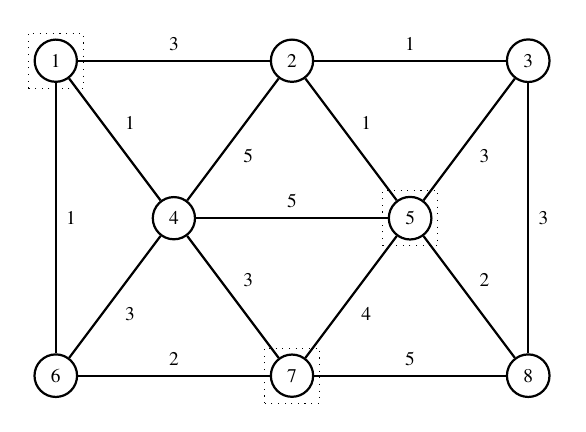
\begin{tikzpicture}
          [font=\scriptsize,
          node/.style={shape=circle,draw=black,fill=white!20, text=black,minimum width=0.5cm,thick},
          arc/.style={-,>=stealth,thick},
          edge/.style={thick}]
          
            \node (1) [node] at (0,2) {1};
            \draw[dotted] (-0.35,1.65) rectangle (0.35,2.35);
            \node (2) [node] at (3,2) {2};
            \node (3) [node] at (6,2) {3};
            \node (4) [node] at (1.5,0) {4};
            \node (5) [node] at (4.5,0) {5};
            \draw[dotted] (4.15,-0.35) rectangle (4.85,0.35);
            \node (6) [node] at (0,-2) {6};
            \node (7) [node] at (3,-2) {7};
            \draw[dotted] (2.65,-2.35) rectangle (3.35,-1.65);
            \node (8) [node] at (6,-2) {8};
 
          %\coordinate (A2) at (2.8,1.75);
          %\coordinate (A3) at (2.8,-1.75);
          %\coordinate (B2) at (3.2,1.75);
          %\coordinate (B3) at (3.2,-1.75);
          
          \draw [arc] (1) to node [auto] {3} (2);
          \draw [arc] (1) to node [auto] {1} (4);
          \draw [arc] (1) to node [auto] {1} (6);
          \draw [arc] (2) to node [auto] {5} (4);
          \draw [arc] (2) to node [auto] {1} (5);
          \draw [arc] (2) to node [auto] {1} (3);
          \draw [arc] (3) to node [auto] {3} (5);
          \draw [arc] (3) to node [auto] {3} (8);
          \draw [arc] (4) to node [auto] {3} (6);
          \draw [arc] (4) to node [auto] {3} (7);
          \draw [arc] (4) to node [auto] {5} (5);
          \draw [arc] (5) to node [auto] {4} (7);
          \draw [arc] (5) to node [auto] {2} (8);
          \draw [arc] (6) to node [auto] {2} (7);
          \draw [arc] (7) to node [auto] {5} (8);

        \end{tikzpicture}
\end{center}

You are consulting for Opstown.  The city council has decided that in order for a fire station to adequately service a citizen location, it must be no more than 3 miles from the customer location (i.e. $D=3$).  The city council has also gathered data on the number of citizens at each customer location $i$, defined as $h_i$, and is providing you with that information in the table below (in hundreds of citizens).  We assume that all ``demand'' can be met by any fire station location.

\vspace{0.25cm}

\begin{tabular}{l|c|c|c|c|c|c|c|c|}
Citizen Location &  1	&	2	&	3	&	4	&
5	&	6	&	7	&	8	
\\
\hline
$h_i$ & 45	&	90	&	110	&	35	&	60	&	105	&	80	&	100	
\end{tabular}

\vspace{.5cm}

\noindent The city council thinks the following decision variables may be useful:
\begin{tabbing}
\noindent{\bf Decision Variables [units]}\\[0.2cm]
\hspace*{.5cm} \= $X_j$ \hspace{1cm} \= 1 if node $j$ is the location of a fire station, 0 otherwise  [binary] \\
\> $Y_{i}$ \> 1 if node $i$ has its ``demand'' satisfied by some fire station, 0 otherwise  [binary] \\ 
\end{tabbing}

{
\blu Facility Location problem
}

\begin{enumerate}
\item The city council would like to know the minimum number of fire stations they need to open.  Using the information above, write an objective function that minimizes the total number of fire stations that need to be opened.

{
\blu
\[
\text{minimize} x_1 + x_5+x_7
\]
}

\item If we define $N_i = \{ j \in J: d_{ij} \leq D \}$ as the neighborhood of $i$, or the set of all fire stations $j$ that can serve customer location $i$.  What is the neighborhood of node 2?
{ \blu
The neighborhood of node $2$ is $\{1,5\}$
}

\item  Write a constraint that ensures that the demand of node 2 is met.  

{
\blu
\[
x_1 + x_5 \geq 1
\]
}

\item  Write a set of constraints in abstract form that ensures that the demand of each customer is met.

{
\blu

\[
\sum_{j \in N_i} x_j \geq 1 \text{ for all $i \in I$}
\]
}


\item  You were able to successfully solve the set covering facility location model, and told the city council they needed to open 2 fire stations.  Based on budget limitations, the city council said they could actually only afford to open a single fire station.  Write a constraint that ensures the total number of open fire stations is equal to one.

{
\blu
\[
x_1 + x_5 + x_7 = 1
\]
}

\item  Because they can only open a single fire station, some citizens will not live close enough to a fire station to be adequately served.  The city council would like to maximize the number of citizens who are adequately covered by the single open fire station.  Using the information above, write an objective function that maximizes the number of citizens covered by the open fire station.
{
\blu
\[
\text{maximize: } \sum_{i \in I} h_i y_i
\]
}

\item  Write a concrete constraint that ensures that the population of location 4 is not included in the count of covered citizens in the objective function if location 4 is not covered by a fire station.

{
\blu
The neighborhood of location 4 is 1 and 7. We can again use our logical constraints approach from number 1 part d. You can do this on your own. The final value we get is:

\[
y_4 \leq x_1 + x_7
\]

}

\item  Write a set of constraints in abstract form that ensure that only covered locations are included in the count of covered citizens in the objective function.

{
\blu

\[
\sum_{j \in N_i} x_j \geq y_i \text{ for all $i \in I$}
\]

}
\end{enumerate}

\newpage

\item Three oil companies (A, B, and C) have submitted bids for satisfying the stated
aviation fuel requirements of four Air Force bases (1, 2, 3, and 4). The table
below displays the fuel requirement of each base, the maximum amount each oil
company can supply to all bases, and the bid each company has made for
supplying each base.\footnote{This problem is a simplification of an actual decision problem
that arose at the United States Department of Defense. The actual problem
involved approximately 300 bases, 100 oil companies, three types of fuels, and
many complicating factors in the bids. Finding the optimal solution to such a
large-scale contract-awards problem required the use of a special-purpose
method. For further details, refer to L.M. Austin and W. W. Hogan, ``Optimizing
the Procurement of Aviation Fuel'', Management Science, Vol. 22, No.5 (January
1976), 515- 527.}

\begin{center}\begin{tabular}{|r|cccc|c|}\hline
    & \multicolumn{4}{c|}{Bids (\$ per 1000 gallons)} & Maximum Supply \\\cline{2-5}
    & Base 1 & Base 2 & Base 3 & Base 4 & (1000 gallons) \\\hline
  Company A & 500 & 600 & 650 & 450 & 50 \\
  Company B & 450 & 300 & 500 & 150 & 40 \\
  Company C & 550 & 450 & 700 & 250 & 60 \\\hline
  Fuel Requirements & 45 & 20 & 30 & 30 & \\
  (1000 gallons) &  &  &  &  & \\\hline
\end{tabular}\end{center}

\begin{enumerate}
\item Formulate an integer program whose solution will allow the bases to satisfy their needs at minimum cost.

{
\blu

For now, this is a standard transportation problem.

\textbf{\underline{Sets}} \\
Let $I$ be the set of companies (supply nodes)\\
Let $J$ be the set of bases (demand nodes)

\textbf{\underline{Decision Variables}} \\

Let $x_{i,j}$ be the units shipped from company $i$ to base $j$ for all $i \in I$ and all $j \in J$

\textbf{\underline{Parameters}} \\

Let $c_{i,j}$ be the cost of shipping from company $i$ to base $j$ for all $i \in I$ and all $j \in J$\\
Let $s_i$ be the supply of company $i$ \\
Let $d_j$ be the demand of base $j$

\begin{optprog*}
\text{min} & \objective{ \sum_{j \in J} \sum_{i \in I} c_{i,j} x_{i,j}  }\\
st & \sum_{i \in I} x_{i,j} & = & d_j & \text{for all $j \in J$} \\
   & \sum_{j \in J} x_{i,j} & = & s_i & \text{for all $i \in I$} \\
   & x_{i,j} & \geq & 0 & \text{for all $i \in I$, $j \in J$}
\end{optprog*}



}

\item Each of the contracts have several complicating factors. We will explore a few of them here.
	\begin{enumerate}
	\item Company A has specified that, for base 1, they must supply either at least 15 thousand gallons to base 1, or it must supply zero gallons to base 1. Add any necessary decision variables and constraints to your model which will satisfy this complicating factor.
	{
	\blu
	Let $y = 1$ if they supply 15,000 gallons to base 1.
	We are trying to enforce that either $x_{1,1} \geq 15$ or $x_{1,1} = 0$. We can achieve this by the following pair of constraints:
	\[
	x_{1,1} \geq 15 y
	\]
	\[
	x_{1,1} \leq 50 y
	\] where $50$ here is taking the place of M	
	
	}	
	
	\item Company B has specified that at least two out of the following three conditions must be satisfied:
		\begin{itemize}
      	\item Supply at most 10 thousand gallons to base 1.
      	\item Supply at least 5 thousand gallons to base 2.
      	\item Supply exactly 7 thousand gallons to base 3.
	    \end{itemize}
	    Add any necessary decision variables and constraints to your model which will satisfy this complicating factor. \emph{Hint: Define a decision variable $y_k$ which $=1$ if condition $k$ is satisfied}.
	    {
	    \blu
		Let $y_k = 1$ if complicating factor $k$ is satisfied.	For the first one, we want to say that, if we satisfy this condition, $x_{2,1} \leq 10$. We can enforce this with 
		\[
		x_{2,1} \leq 10 + 40 (1-y_1)
		\]
		
		If we enforce this, this constraint becomes $x_{2,1} \leq 10$. If not $y_1 = 0$ and it defaults to an upper bound.
		
		For condition 2, we want to say that $x_{2,2} \geq 5$ if $y_2 = 1$. We can enforce this with:
		\[
		x_{2,2} \geq 5 y_2
		\]
		
		If $y_2 = 1$, we enforce this. If $y_2 = 0$, we do not and it defaults to non-negativity.
		
		For condition 3, we want $x_{2,3} = 7$ if $y_3 = 1$. There's a common mistake here of setting this as $x_{2,3} = 7y$. THIS DOES NOT WORK. Instead, we can do the following pair:
		\[
		x_{2,3} \leq 7 + 40 (1-y_3)
		\]
		\[
		x_{2,3} \geq 7 y_3
		\]

		If $y_3 = 1$, the two constraints becomes $x_{2,3} \leq 7$ and $x_{2,3} \geq 7$ which means $x_{2,3} = 7$. If $y_3 = 0$, the first constraint becomes a non-binding upper bound and the second becomes non-negativity.		

		Finally, it says at least two must be satisfied. So we add:
		\[
		y_1 + y_2 + y_3 \geq 2
		\]		
		
	    }
	  \item Company C has specified that if it supplies more than 15 thousand gallons to base 1, then it must supply at least 20 thousand gallons to base 2. Add any necessary decision variables and constraints to your model which will satisfy this complicating factor.
	  {
	  \blu
	In this one we want that if $x_{3,1} \geq 15$ then $x_{3,2} \geq 20$. This one is tough, because the obvious answer doesn't work. Instead, we need to upper bound $x_{3,1}$ and say that if $x_{3,1}$ is less than 15 then $x_{3,2}$ must also be less than 20. We can do this as follows:
	\[
	x_{3,1} \leq 15 + 60 y_3
	\]
	\[
	x_{3,2} \geq 20 - 60 (1-y_3)
	\]
	  
	  So if $y_3 = 1$, we enforce this constraint. The first becomes $x_{3,1} \leq 75$ (letting it exceed 15) and the second becomes $x_{3,2} \geq 20$. If $y_3 = 0$, $x_{3,1}$ is less than 15 and $x_{3,2}$ is free.
	  }
	\end{enumerate}
\end{enumerate}

\newpage
\item The final exam period at USNA runs through 7 days starting on Tuesday Dec 13. Suppose you're trying to help the math department schedule their final exams. The table below lists 8 courses you'd want to schedule. A 1 in the table indicates that these two courses are usually taken at the same time (for example SA405 and SA402 are usually taken by the same group of students so a 1 is placed in their corresponding rows/columns).

\begin{center}\begin{tabular}{|c|cccccccc|}\hline
      & SA405 & SA402 & SA430 & SM261 & SM233 & SM239 & SA421 & SM342 \\ \hline
SA405 &       & 1     & 1     &       &       &       &       & 1      \\
SA402 & 1     &       & 1     &       &       &       &       & 1     \\
SA430 & 1     & 1     &       &       &       &       &       & 1     \\
SM261 &       &       &       &       & 1     &  1    &       &       \\
SM233 &       &       &       & 1     &       &  1    &       &       \\
SM239 &       &       &       & 1     & 1     &       &       &       \\
SA421 &       &       &       &       &       &       &       & 1     \\
SM342 & 1     &  1    & 1     &       &       &       &  1    &       \\ \hline
\end{tabular}\end{center}

Suppose that the math department wants to schedule the exams for these classes during the first 3 days of exam week. Each exam can be scheduled to begin at either 800, 1200, or 1600. Note that at any time period in any day, a maximum of two exams can occur.

Suppose we define the following three sets:

$C$ is the set of classes $C = \{\text{SA405, SA402, ...}\}$ \\
$D$ is the set of days $D = \{1,2,3\}$ \\
$S$ is the set of starting times for the exams $S = \{8,12,16\}$

Lastly, we define the variables:

Let $x_{c,d,s} = 1$ if class $c$ is scheduled to take its exam on day $d$ during time period $s$ for all $c \in C$, $d \in D$, and $s \in S$.

Formulate a parameterized integer program which maximizes the number of exams beginning at time 8. Make sure you include constraints that prevent any exams with overlapping students from two classes from occurring at the same time.

{\blu

\textbf{\underline{Parameters}}

Let $a_{i,j} = 1$ if class $i$ overlaps with class $j$ for all $i \in C$ and $j \in C$ and 0 otherwise.

\textbf{\underline{Objective Function}}
\[
\text{max } \sum_{c \in C} \sum_{d \in D} x_{c,d,8}
\]

\textbf{\underline{Constraints}}

\begin{optprog*}
& \sum_{d \in D} \sum_{s \in S} x_{c,d,s} & = & 1 & \text{for all $c \in C$} & \text{(each exam is scheduled)} \\
& \sum_{c \in C} \sum_{d \in D} x_{c,d,s} & \leq & 2 & \text{for all $s \in S$} & \text{(2 exams per time period max)} \\
& x_{i,d,s} + x_{j,d,s} & \leq & 2 - a_{i,j} & \text{for all $i \in C$, $j \in C$, $d \in D$, $s \in S$} & \text{(no overlapping exams)} \\
& x_{c,d,s} & \in & \{0,1\} & \text{for all $c \in C$, $d \in D$, $s \in S$} & \text{(binary)}
\end{optprog*}

}


\end{enumerate}
\end{document}
